% !TEX root = ../ComputationalOTFnT.tex
\newcommand{\myFigRKHS}[1]{\includegraphics[width=.195\linewidth]{rkhs/#1}}
\chapter{Statistical Divergences}
\label{c-statistical}

We study in this chapter the statistical properties of the Wasserstein distance. More specifically, we compare it to other major distances and divergences routinely used in data sciences. We quantify how one can approximate the distance between two probability distributions when having only access to samples from said distributions. To introduce these subjects,~\S\ref{sec-phi-div} and~\S\ref{sec-dual-norms} review respectively divergences and integral probability metrics between probability distributions. A divergence $D$ typically satisfies $D(\al,\be) \geq 0$ and $D(\al,\be)=0$ if and only if $\al=\be$, but it does not need to be symmetric or satisfy the triangular inequality. An integral probability metric for measures is a dual norm defined using a prescribed family of test functions. These quantities are sound alternatives to Wasserstein distances and are routinely used as loss functions to tackle inference problems, as will be covered in~\S\ref{c-variational}. We show first in~\S\ref{sec-non-embeddability} that the optimal transport distance is not Hilbertian, \ie one cannot approximate it efficiently using a Hilbertian metric on a suitable feature representation of probability measures. We show in \S\ref{sec-empirical-wass} how to approximate $D(\al,\be)$ from discrete samples $(x_i)_i$ and $(y_j)_j$ drawn from $\al$ and $\be$. A good statistical understanding of that problem is crucial when using the Wasserstein distance in machine learning. Note that this section will be chiefly concerned with the statistical approximation of optimal transport between distributions supported on \emph{continuous} sets. The very same problem when the ground space is finite has received some attention in the literature following the work of~\citet{sommerfeld2018inference}, extended to entropic regularized quantities by~\citet{bigot2017central}.


%%%%%%%%%%%%%%%%%%%%%%%%%%%%%%%%%%%%%%%%%%%%%%%%%%%%%%%%%%%%%%%%%%%%%%%%%%%%%%%%%%%%%%%%%%%%%%%%%%%%
%%%%%%%%%%%%%%%%%%%%%%%%%%%%%%%%%%%%%%%%%%%%%%%%%%%%%%%%%%%%%%%%%%%%%%%%%%%%%%%%%%%%%%%%%%%%%%%%%%%%
%%%%%%%%%%%%%%%%%%%%%%%%%%%%%%%%%%%%%%%%%%%%%%%%%%%%%%%%%%%%%%%%%%%%%%%%%%%%%%%%%%%%%%%%%%%%%%%%%%%%
\section{$\phi$-Divergences}
\label{sec-phi-div}

Before detailing in the following section ``weak'' norms, whose construction shares similarities with $\Wass_1$, let us detail a generic construction of so-called divergences between measures, which can then be used as loss functions when estimating probability distributions. Such divergences compare two input measures by comparing their mass \emph{pointwise}, without introducing any notion of mass transportation. Divergences are functionals which, by looking at the pointwise ratio between two measures, give a sense of how close they are. They have nice analytical and computational properties and build  upon \emph{entropy functions}.

\begin{defn}[Entropy function]
\label{def_entropy}
A function $\phi : \RR \to \RR \cup \{\infty\}$ is an entropy function if it is lower semicontinuous, convex, $\dom \phi\subset [0,\infty[$, and satisfies the following feasibility condition:  $\dom \phi \; \cap\;  ]0, \infty[\; \neq \emptyset$. The speed of growth of $\phi$ at $\infty$ is described by %its recession (or horizon) function
\eq{
\phi'_\infty = \lim_{x\rightarrow +\infty} \varphi(x)/x \in \RR \cup \{\infty\} \, .
}
\end{defn}

If $\phi'_\infty = \infty$, then $\phi$ grows faster than any linear function and $\phi$ is said \emph{superlinear}. Any entropy function $\phi$ induces a $\phi$-divergence (also known as Cisz\'ar divergence~\citep{ciszar1967information,ali1966general} or $f$-divergence) as follows.



\begin{defn}[$\phi$-Divergences]
\label{def_divergence}
Let $\phi$ be an entropy function.
For $\al,\be \in \Mm(\X)$, let $\frac{\d \al}{\d \be} \be + \al^{\perp}$ be the Lebesgue decomposition\footnote{The Lebesgue decomposition theorem asserts that, given $\be$, $\al$ admits a unique decomposition as the sum of two measures $\al^s + \al^\perp$ such that $\al^s$ is absolutely continuous with respect to $\be$ and $\al^\perp$ and $\be$ are singular.} of $\al$ with respect to $\be$. The divergence $\Divergm_\phi$ is defined by
\eql{\label{eq-phi-div}
	\Divergm_\phi (\al|\be) \eqdef \int_\X \phi\left(\frac{\d \al}{\d \be} \right) \d \be 
+ \phi'_\infty \al^{\perp}(\X)
}
if $\al,\be$ are nonnegative and $\infty$ otherwise.
\end{defn}%

The additional term $\phi'_\infty \al^{\perp}(\X)$ in~\eqref{eq-phi-div} is important to ensure that $\Divergm_\phi$ defines a continuous functional (for the weak topology of measures) even if $\phi$ has a linear growth at infinity, as this is, for instance, the case for the absolute value~\eqref{eq-tv-entropy} defining the TV norm. If $\phi$ as a superlinear growth, \eg the usual entropy~\eqref{eq-shannon-entropy}, then $\phi'_\infty=+\infty$ so that $\Divergm_\phi (\al|\be) = +\infty$ if $\al$ does not have a density with respect to $\be$. 

In the discrete setting, assuming 
\eql{\label{eq-div-disc-meas}
	\al=\sum_i \a_i \de_{x_i}
	\qandq \be=\sum_i \b_i \de_{x_i}
} 
are supported on the same set of $n$ points $(x_i)_{i=1}^n \subset \X$,~\eqref{eq-phi-div} defines a divergence on $\simplex_n$
\eql{\label{eq-discr-diverg}
	\DivergmD_\phi(\a|\b) = \sum_{i \in \Supp(\b)} \phi\pa{ \frac{\a_i}{\b_i} } \b_i + \phi'_\infty \sum_{i \notin \Supp(\b)} \a_i,
}
where $\Supp(\b) \eqdef \enscond{i \in \range{n}}{ b_i \neq 0 }$.

The proof of the following proposition can be found in~\cite[Thm 2.7]{LieroMielkeSavareLong}.

\begin{proposition}
If $\phi$ is an entropy function, then $\Divergm_\phi$ is jointly $1$-homogeneous, convex and weakly* lower semicontinuous in $(\al,\be)$.
\end{proposition}


\begin{figure}[h!]
\centering
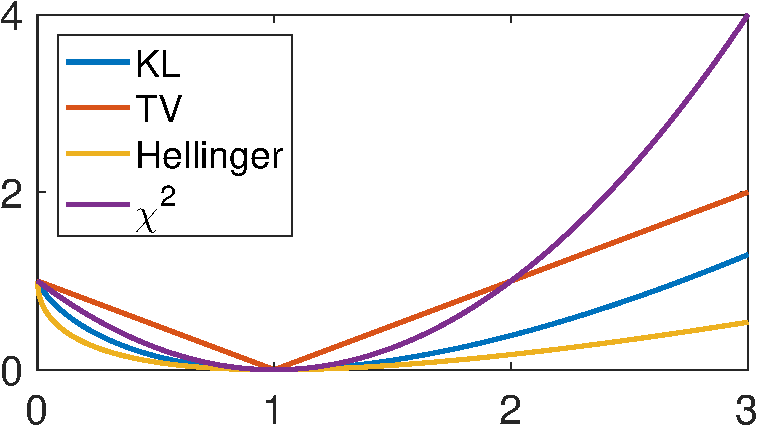
\includegraphics[width=.6\linewidth]{divergences/divergences}
\caption{\label{fig-divergences}
Example of entropy functionals.
}
\end{figure}


\begin{rem}[Dual expression]
	A $\phi$-divergence can be expressed using the Legendre transform 
	\eq{
		\phi^*(s) \eqdef \usup{t \in \RR} st - \phi(t)
	}
	of $\phi$ (see also~\eqref{eq-legendre}) as
	\eq{
		\Divergm_\phi (\al|\be) = \usup{f: \X \rightarrow \RR} \int_\X f(x) \d\al(x) - \int_\X \phi^*(f(x)) \d\be(x); 
	}
	see~\citet{LieroMielkeSavareLong} for more details.
\end{rem}


We now review a few popular instances of this framework. Figure~\ref{fig-divergences} displays the associated entropy functionals, while Figure~\ref{fig-divergences-relations} reviews the relationship between them.





\begin{figure}[h!]
\centering
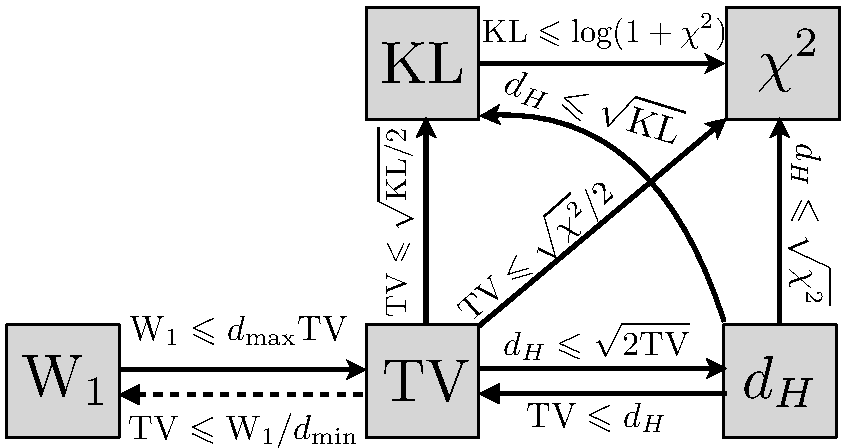
\includegraphics[width=.6\linewidth]{divergences/divergences-comparison}
\caption{\label{fig-divergences-relations}
Diagram of relationship between divergences (inspired by~\citet{gibbs2002choosing}).
For $\X$ a metric space with ground distance $d$, $d_{\max} = \sup_{(x,x')} d(x,x')$ is the diameter of $\X$. When $\X$ is discrete, $d_{\min} \eqdef \min_{x \neq x'} d(x,x')$. \todoK{Tripple check these bounds since they might use different definition/normalization. }\todoK{Change the notation for the Hellinger distance one the symbol is decided $\Hellinger$. }
}
\end{figure}


\begin{example}[Kullback--Leibler divergence]
\label{ex_KLdiv}
The Kullback--Leibler divergence $\KL \eqdef \Divergm_{\phi_{\KL}}$, also known as the relative entropy, was already introduced in~\eqref{eq-defn-rel-entropy} and~\eqref{eq-kl-defn}. It is the divergence associated to the Shannon--Boltzman entropy function $\phi_{\KL}$, given by
\eql{\label{eq-shannon-entropy}
	\phi_{\KL}(s)= \begin{cases}
		s\log(s)-s+1 & \textnormal{for } s>0 , \\
		1 & \textnormal{for } s=0 , \\
		+\infty & \textnormal{otherwise.}
		\end{cases}
}
\end{example}

\begin{remark}[Bregman divergence]\label{rem-bregman}
The discrete KL divergence, $\KLD \eqdef \DivergmD_{\phi_{\KL}}$, has the unique property of being both a $\phi$-divergence and a Bregman divergence.
%
For discrete vectors in $\RR^n$, a Bregman divergence~\citep{bregman1967relaxation} associated to a smooth strictly convex function $\psi : \RR^n \rightarrow \RR$ is defined as
\eql{\label{eq-bregman-discr}
	\VectMode{B}_\psi(\a|\b) \eqdef \psi(\a) - \psi(\b) - \dotp{\nabla \psi(\b)}{\a-\b}, 
}
where $\dotp{\cdot}{\cdot}$ is the canonical inner product on $\RR^n$. Note that $\VectMode{B}_\psi(\a|\b)$ is a convex function of $\a$ and a linear function of $\psi$.
%
Similarly to $\phi$-divergence, a Bregman divergence satisfies $\VectMode{B}_\psi(\a|\b) \geq 0$ and $\VectMode{B}_\psi(\a|\b)=0$ if and only if $\a=\b$. 
%
The KL divergence is the Bregman divergence for minus the entropy $\psi = -\HD$ defined in~\eqref{eq-discr-entropy}), \ie $\KLD = \VectMode{B}_{-\HD}$. 
%
A Bregman divergence is locally a squared Euclidean distance since
\eq{
	\VectMode{B}_\psi(\a + \varepsilon|\a + \eta) = \dotp{ \partial^2 \psi(\a)(\varepsilon-\eta) }{\varepsilon-\eta}
	+ o(\norm{\varepsilon-\eta}^2)
}
and the set of separating points $\enscond{\a}{\VectMode{B}_\psi(\a|\b) = \VectMode{B}_\psi(\a|\b')}$ is a hyperplane between $\b$ and $\b'$.
%
These properties make Bregman divergence suitable to replace Euclidean distances in first order optimization methods. The best know example is mirror gradient descent~\citep{beck2003mirror}, which is an explicit descent step of the form~\eqref{eq-explicit-metricflow}.
%
Bregman divergences are also important in convex optimization and can be used, for instance, to derive Sinkhorn iterations and study its convergence in finite dimension; see Remark~\ref{rem-iterative-projection}.
%%%% Should be re-written in infinite dimension
%While KL is both a $\phi$ and a Bregman divergence, these are radically different concepts. In particular, to generalize formula~\eqref{eq-bregman-discr} to nondiscrete measures on some space $\Xx$, one needs to fix a reference measure $\xi$ and consider only measures $\al,\be$ with square integrable densities $\frac{\d\al}{\d\xi},\frac{\d\be}{\d\xi} \in L^2(\d\xi)$. For some strictly convex $\psi : L^2(\d\xi) \rightarrow \RR$, one then defines the Bregman divergence as 
%\eq{
%	\Bb_{\psi,\xi}(\al|\be) \eqdef \psi\pa{\frac{\d\al}{\d\xi}} - 
%		\psi\pa{\frac{\d\be}{\d\xi}} - 
%		\int_{\X} \eta(x) \pa{ 
%			\frac{\d\al}{\d\xi}(x)-\frac{\d\be}{\d\xi}(x)
%		} \d \xi(x),
%}
%where $\eta = \nabla \psi\pa{\frac{\d\be}{\d\xi}}  \in L^2(\d\xi)$ is the gradient~\citep{rao1985cross,jones1990general}.  
%%% 
%The simplest case is if $\psi(\rho) = \int_\X \tilde\psi(\rho(x)) \d\xi(x)$ in which case
%\eq{
%	\Bb_{\psi,\xi}(\al|\be) \eqdef 
%		\int_\X \pa{
%		\tilde\psi\pa{\frac{\d\al}{\d\xi}} - 
%		\tilde\psi\pa{\frac{\d\be}{\d\xi}} - 
%		\tilde\psi'\pa{\frac{\d\be}{\d\xi}}
%		\pa{
%			\frac{\d\al}{\d\xi}-\frac{\d\be}{\d\xi}
%		}
%		} \d \xi.
%}
\end{remark}

\begin{remark}[Hyperbolic geometry of KL]
	It is interesting to contrast the geometry of the Kullback--Leibler divergence to that defined by quadratic optimal transport when comparing Gaussians. As detailed, for instance, by~\citet{costa2015fisher}, the Kullback--Leibler divergence has a closed form for Gaussian densities. In the univariate case, $\dim=1$, if $\al = \Nn(m_\al,\si_\al^2)$ and $\be = \Nn(m_\be,\si_\be^2)$, one has
	\eql{\label{eq-kl-gaussian}
		\KL(\al|\be) = \frac{1}{2}\pa{
			\frac{\si_\al^2}{\si_\be^2}  + 
			\log\pa{\frac{\si_\be^2}{\si_\al^2}}
			+ \frac{|m_\al-m_\be|}{\si_\be^2}
			 - 1
		}.
	}	
	This expression shows that the divergence between $\al$ and $\be$ diverges to infinity as $\si_\be$ diminishes to $0$ and $\be$ becomes a Dirac mass. In that sense, one can say that singular Gaussians are infinitely far from all other Gaussians in the KL geometry. That geometry is thus useful when one wants to avoid dealing with singular covariances. To simplify the analysis, one can look at the infinitesimal geometry of KL, which is obtained by performing a Taylor expansion at order 2,
	\eq{
		\KL( \Nn(m+\de_m,(\si+\de_\si)^2) | \Nn(m,\si^2) ) = \frac{1}{\si^2}\pa{
			\frac{1}{2}\de_m^2 + \de_\si^2
		} + 
		o( \de_m^2,\de_\si^2 ).
	}
	This local Riemannian metric, the so-called Fisher metric, expressed over $(m/\sqrt{2},\si) \in \RR \times \RR_{+,*}$, matches exactly that of the hyperbolic Poincar\'e half plane. 
	%
	Geodesics over this space are half circles centered along the $\si=0$ line and have an exponential speed, \ie they only reach the limit $\si=0$ after an infinite time. 
	%
	Note in particular that if $\si_\al=\si_\be$ but $m_\al \neq m_\al$, then the geodesic between $(\al,\be)$ over this hyperbolic half plane does not have a constant standard deviation. 
	
	The KL hyperbolic geometry over the space of Gaussian parameters $(m,\si)$ should be contrasted with the Euclidean geometry associated to OT as described in Remark~\ref{rem-dist-gaussians}, since in the univariate case
	\eql{\label{eq-univariate-gauss}
		\Wass_2^2( \al,\be ) = |m_\al - m_\be |^2 + |\si_\al-\si_\be|^2. 
	}  
	Figure~\ref{fig-kl-gaussians} shows a visual comparison of these two geometries and their respective geodesics.
	%
	This interesting comparison was suggested to us by Jean Feydy.  
\end{remark}



\begin{figure}[h!]
\centering
\begin{tabular}{@{}c@{\hspace{3mm}}c@{}}
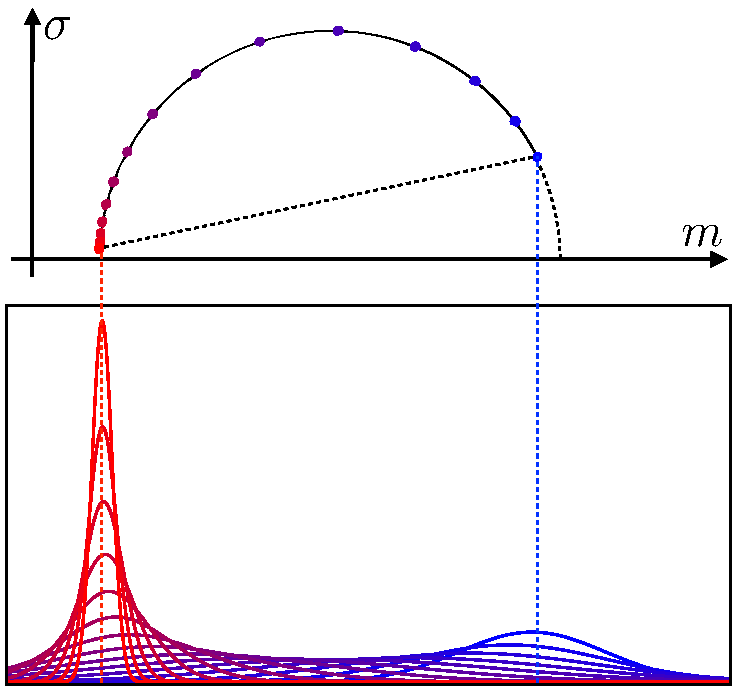
\includegraphics[width=.45\linewidth]{kl-gaussian/interp-kl}&
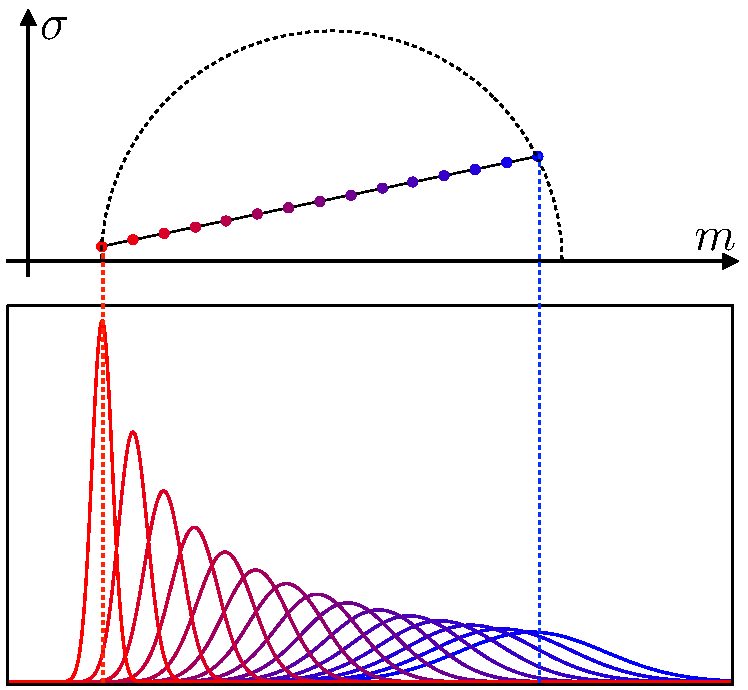
\includegraphics[width=.46\linewidth]{kl-gaussian/interp-ot}\\
KL & OT
\end{tabular}
\caption{\label{fig-kl-gaussians}
Comparisons of interpolation between Gaussians using KL (hyperbolic) and OT (Euclidean) geometries.
}
\end{figure}


\begin{example}[Total variation]\label{exmp-tv}
The total variation distance $\TV \eqdef \Divergm_{\phi_{\TV}}$ is the divergence associated to
\eql{\label{eq-tv-entropy}
	\phi_{\TV}(s)= \begin{cases}
		|s-1| & \textnormal{for } s\geq0 , \\
		+\infty & \textnormal{otherwise.}
		\end{cases}
}
It actually defines a norm on the full space of measure $\Mm(\X)$ where
\eql{\label{eq-defn-tv}
	\TV(\al|\be) = \norm{\al-\be}_{\TV},
	\qwhereq
	\norm{\al}_{\TV} = |\al|(\X) = \int_\X \d|\al|(x).
}
If $\al$ has a density $\density{\al}$ on $\X=\RR^\dim$, then the TV norm is the $L^1$ norm on functions, $\norm{\al}_{\TV} = \int_\X |\density{\al}(x)| \d x = \norm{\density{\al}}_{L^1}$.
%
If $\al$ is discrete as in~\eqref{eq-div-disc-meas}, then the TV norm is the $\ell^1$ norm of vectors in $\RR^n$, $\norm{\al}_{\TV}=\sum_i |\a_i| = \norm{\a}_{\ell^1}$.
\end{example}

\begin{rem}[Strong vs. weak topology]
	The total variation norm~\eqref{eq-defn-tv} defines the so-called ``strong'' topology on the space of measure. 
	%
	On a compact domain $\X$ of radius $R$, one has 
	\eq{
		\Wass_1(\al,\be) \leq R \norm{\al-\be}_{\TV}
	}
	so that this strong notion of convergence implies the weak convergence metrized by Wasserstein distances. 
	%
	The converse is, however, not true, since $\de_x$ does not converge strongly to $\de_y$ if $x \rightarrow y$ (note that
	$\norm{\de_x-\de_y}_{\TV}=2$ if $x \neq y$). 
	%
	A chief advantage is that $\Mm_+^1(\Xx)$ (once again on a compact ground space $\X$) is compact for the weak topology, so that from any sequence of probability measures $(\al_k)_k$, one can always extract a converging subsequence, which makes it a suitable space for several optimization problems, such as those considered in Chapter~\ref{c-variational}.
\end{rem}


\begin{example}[Hellinger]\label{exmp-hellinger}
	The Hellinger distance $\Hellinger \eqdef \Divergm_{\phi_{H}}^{1/2}$ is the square root of the divergence associated to
	\eq{
		\phi_{H}(s)= \begin{cases}
			|\sqrt{s}-1|^2 & \textnormal{for } s\geq0 , \\
			+\infty & \textnormal{otherwise.}
			\end{cases}
	}
	As its name suggests, $\Hellinger$ is a distance on $\Mm_+(\X)$, which metrizes the strong topology as $\norm{\cdot}_{\TV}$. 
	%
	If $(\al,\be)$ have densities $(\density{\al},\density{\be})$ on $\X=\RR^\dim$, then $\Hellinger(\al,\be) = \norms{\sqrt{\density{\al}}-\sqrt{\density{\be}}}_{L^2}$.
	%
	If $(\al,\be)$ are discrete as in~\eqref{eq-div-disc-meas}, then $\Hellinger(\al,\be) = \norms{\sqrt{\a}-\sqrt{\b}}$.	
	%
	Considering $\phi_{L^p}(s)=|s^{1/p}-1|^p$ generalizes the Hellinger ($p=2$) and total variation ($p=1$) distances
	and $\Divergm_{\phi_{L^p}}^{1/p}$ is a distance which metrizes the strong convergence for $0<p<+\infty$. 
\end{example}


\begin{example}[Jensen--Shannon distance]
	The KL divergence is not symmetric and, while being a Bregman divergence (which are locally quadratic norms), it is not the square of a distance. On the other hand, the Jensen--Shannon distance $\text{JS}(\al,\be)$, defined as
	\eq{
		\text{JS}(\al,\be)^2 \eqdef \frac{1}{2}\pa{
			\KL(\al|\xi) + \KL(\be|\xi)
		}
		\qwhereq
		\xi = \frac{\al+\be}{2}, 
	}
	is a distance~\citep{endres2003new,osterreicher2003new}. 
	% 
	$\text{JS}^2$ can be shown to be a $\phi$-divergence for $\phi(s) = t\log(t)-(t+1)\log(t+1)$.
	%
	In sharp contrast with $\KL$, $\text{JS}(\al,\be)$ is always bounded; more precisely, it satisfies $0 \leq \text{JS}(\al,\be)^2 \leq \ln(2)$. 
	%
	Similarly to the TV norm and the Hellinger distance, it metrizes the strong convergence. 
\end{example}



\begin{example}[$\chi^2$]\label{exmp-chisquare}
	The $\chi^2$-divergence $\chi^2 \eqdef \Divergm_{\phi_{\chi^2}}$ is the divergence associated to
	\eq{
		\phi_{\chi^2}(s)= \begin{cases}
			|s-1|^2 & \textnormal{for } s\geq0 , \\
			+\infty & \textnormal{otherwise.}
			\end{cases}
	}
	If $(\al,\be)$ are discrete as in~\eqref{eq-div-disc-meas} and have the same support, then 
	\eq{
		\chi^2(\al|\be) = \sum_i \frac{(\a_i-\b_i)^2}{\b_i}.
	}	
\end{example}


%%%%%%%%%%%%%%%%%%%%%%%%%%%%%%%%%%%%%%%%%%%%%%%%%%%%%%%%%%%%%%%%%%%%%%%%%%%%%%%%%%%%%%%%%%%%%%%%%%%%
%%%%%%%%%%%%%%%%%%%%%%%%%%%%%%%%%%%%%%%%%%%%%%%%%%%%%%%%%%%%%%%%%%%%%%%%%%%%%%%%%%%%%%%%%%%%%%%%%%%%
%%%%%%%%%%%%%%%%%%%%%%%%%%%%%%%%%%%%%%%%%%%%%%%%%%%%%%%%%%%%%%%%%%%%%%%%%%%%%%%%%%%%%%%%%%%%%%%%%%%%
\section{Integral Probability Metrics}
\label{sec-dual-norms}


Formulation~\eqref{eq-w1-cont} is a special case of a dual norm. A dual norm is a convenient way to design ``weak'' norms that can deal with arbitrary measures. For a symmetric convex set $B$ of measurable functions, one defines 
\eql{\label{eq-dual-norm-cont}
	\norm{\al}_B \eqdef 
	\umax{\f} \enscond{ \int_{\X} \f(x) \d\al(x) }{ \f \in B}.
}
These dual norms are often called ``integral probability metrics'; see~\citep{sriperumbudur2012empirical}.

 
% Cf. ``Integral probability metrics and their generating classes of functions".  

\begin{example}[Total variation]
The total variation norm (Example~\ref{exmp-tv}) is a dual norm associated to the whole space of continuous functions
\eq{
	B = \enscond{f \in \Cc(\X)}{\norm{f}_\infty \leq 1}.
}
The total variation distance is the only nontrivial divergence that is also a dual norm; see~\citep{sriperumbudur2009integral}. 
\end{example}

\begin{rem}[Metrizing the weak convergence]\label{rem-ipm-weak}
By using smaller ``balls'' $B$, which typically only contain continuous (and sometimes regular) functions, one defines weaker dual norms.
%
In order for $\norm{\cdot}_B$ to metrize the weak convergence (see Definition~\ref{dfn-weak-conv}), it is sufficient for the space spanned by $B$ to be dense in the set of continuous functions for the sup-norm $\norm{\cdot}_\infty$ (i.e. for the topology of uniform convergence); see~\citep[para. 5.1]{ambrosio2006gradient}.
\end{rem}

Figure~\ref{fig-dual-norms} displays a comparison of several such dual norms, which we now detail.


\begin{figure}[h!]
\centering
\begin{tabular}{@{}c@{\hspace{3mm}}c@{}}
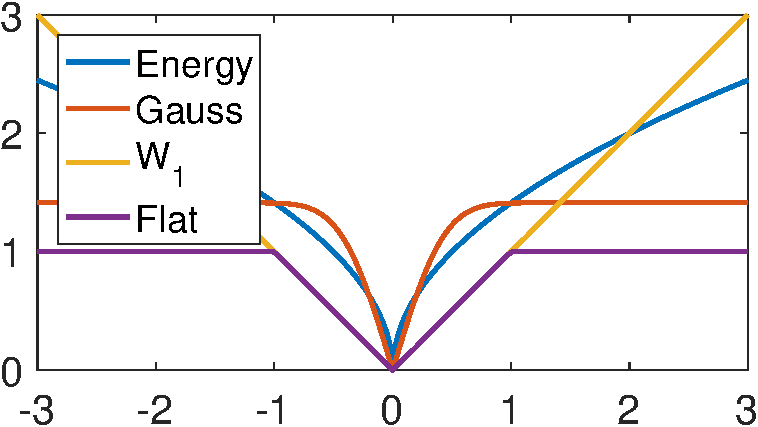
\includegraphics[width=.45\linewidth]{dual-norms/1dirac-1dirac} &
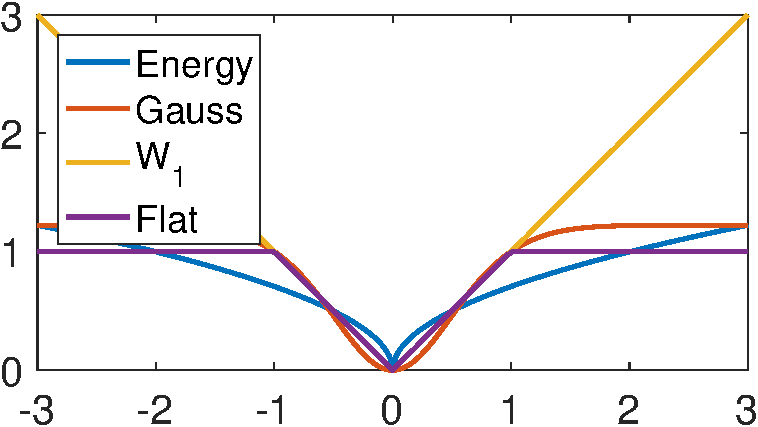
\includegraphics[width=.45\linewidth]{dual-norms/1dirac-2dirac} \\
$(\al,\be)=(\de_0,\de_t)$ &
$(\al,\be)=(\de_0,\frac{1}{2}(\de_{-t/2}+\de_{t/2}))$
\end{tabular}
\caption{\label{fig-dual-norms}
Comparison of dual norms. 
}
\end{figure}



%%%%
\subsection{$\Wass_1$ and Flat Norm}

If the set $B$ is bounded, then $\norm{\cdot}_B$ is a norm on the whole space $\Mm(\Xx)$ of measures.
%
This is not the case of $\Wass_1$, which is only defined for $\al$ such that $\int_\X \d\al=0$ (otherwise $\norm{\al}_B=+\infty$). 
%
This can be alleviated by imposing a bound on the value of the potential $\f$, in order to define for instance the flat norm.

\begin{example}[$\Wass_1$ norm]
$\Wass_1$ as defined in~\eqref{eq-w1-cont}, is a special case of dual norm~\eqref{eq-dual-norm-cont}, using
\eq{ 
	B = \enscond{f}{\Lip(f) \leq 1}
} 
the set of 1-Lipschitz functions.
\end{example}

\begin{example}[Flat norm and Dudley metric]
The flat norm is defined using 
\eql{\label{eq-set-flatnorm}
	B=\enscond{f}{\norm{\nabla \f}_\infty \leq 1 \qandq \norm{\f}_\infty \leq 1}.
}
It metrizes the weak convergence on the whole space $\Mm(\X)$.
% 
Formula~\eqref{eq-w1-discr} is extended to compute the flat norm by adding the constraint $\abs{\fD_k} \leq 1$.
%
The flat norm is sometimes called the ``Kantorovich--Rubinstein'' norm~\citep{hanin1992kantorovich} and has been used as a fidelity term for inverse problems in imaging~\citep{lellmann2014imaging}.
%
The flat norm is  similar to the Dudley metric, which uses
\eq{\label{eq-set-dudley}
	B=\enscond{f}{\norm{\nabla \f}_\infty + \norm{\f}_\infty \leq 1}.
}
\end{example}


%%%%
\subsection{Dual RKHS Norms and Maximum Mean Discrepancies}
\label{sec-mmd}


It is also possible to define ``Euclidean'' norms (built using quadratic functionals) on measures using the machinery of kernel methods and more specifically reproducing kernel Hilbert spaces (RKHS; see~\citep{scholkopf2002learning} for a survey of their applications in data sciences), of which we recall first some basic definitions.

\begin{defn}\label{def-negativedefinitekernel}
A symmetric function $k$ (resp., $\varphi$) defined on a set $\X \times \X$ is said to be positive (resp., negative) definite if for any $n\geq0$, family $x_1,\dots,x_n\in\Z$, and vector $r\in\RR^n$ the following inequality holds:
\eql{\label{eq-dual-kern}
	\sum_{i,j=1}^n r_i r_j k(x_i,x_j)\geq 0, 
	\quad
	\left(\text{resp.}\quad\sum_{i,j=1}^n r_i r_j \varphi(x_i,x_j)\leq 0\right).
}
The kernel is said to be conditionally positive if positivity only holds in~\eqref{eq-dual-kern} for zero mean vectors $r$ (i.e. such that $\dotp{r}{\ones_n}=0$).  
\end{defn}


\if 0 %%%% REMOVED 
Using a positive definite kernel $k$, one can now define a Hilbertian norm $\norm{\cdot}_\Krkhs$ on functions 
\eq{
	\norm{f}_\Krkhs^2 \eqdef \int_{\X \times \X} \Krkhs(x,y) f(x) f(y) \d \rho(x) \d \rho(y)
}
where $\rho$ is some reference measure, typically Lebesgue's measure on $\X=\RR^\dim$. This norm can then be used to define a subset $B$ of functions with bounded RKHS norm,
\eql{\label{eq-dual-rkhs}
	B = \enscond{\f}{ \norm{\f}_\Krkhs \leq 1}
}
%
that is plugged into notation~\eqref{eq-dual-norm-cont}. The dual RKHS norm for measures that results from this construction is often referred to as the ``maximum mean discrepancy'' (MMD) (see~\citet{gretton2007kernel}), and can be revisited through the prism of Kernel Mean Embeddings (see~\citet{muandet2017kernel} for a review). 
\fi 


If $k$ is conditionally positive, one defines the following norm:  
\eql{\label{eq-kernel-dual}
	\norm{\al}^2_{\Krkhs} \eqdef \int_{\X \times \X} \Krkhs(x,y) \d \al(x) \d \al(y). 
}
These norms are often referred to as ``maximum mean discrepancy'' (MMD) (see~\citep{gretton2007kernel}) and have also been called ``kernel norms'' in shape analysis~\citep{glaunes2004diffeomorphic}.
%
This expression~\eqref{eq-kernel-dual} can be rephrased, introducing two independent random vectors $(X,X')$ on $\X$ distributed with law $\al$, as
\eq{
	\norm{\al}^2_{\Krkhs} = \EE_{X,X'}( \Krkhs(X,X') ). 
}
One can show that $\norm{\cdot}^2_{\Krkhs}$ is the dual norm in the sense of~\eqref{eq-dual-norm-cont} associated to the unit ball $B$ of the RKHS associated to $k$. We refer to~\citep{berlinet03reproducing,Hofmann2008,scholkopf2002learning} for more details on RKHS functional spaces.  

\begin{rem}[Universal kernels]
According to Remark~\ref{rem-ipm-weak}, the MMD norm $\norm{\cdot}_k$ metrizes the weak convergence if the span of the dual ball $B$ is dense in the space of continuous functions $\Cc(\Xx)$. This means that finite sums of the form $\sum_{i=1}^n a_i k(x_i,\cdot)$ (for arbitrary choice of $n$ and points $(x_i)_i$) are dense in $\Cc(\Xx)$ for the uniform norm $\norm{\cdot}_\infty$.  For translation-invariant kernels over $\X=\RR^d$, $\Krkhs(x,y)=\Krkhs_0(x-y)$, this is equivalent to having a nonvanishing Fourier transform, $\hat \Krkhs_0(\om) >0$.
\end{rem}

In the special case where $\al$ is a discrete measure of the form~\eqref{eq-pair-discr}, one thus has the simple expression
\eq{
	\norm{\al}_{\Krkhs}^2 = \sum_{i=1}^n \sum_{i'=1}^n \a_i\a_{i'} \KrkhsD_{i,i'}  = \dotp{\KrkhsD\a}{\a}
	\qwhereq
	\KrkhsD_{i,i'} \eqdef \Krkhs(x_i,x_{i'}).
}
In particular, when $\al=\sum_{i=1}^n \a_i \de_{x_i}$ and $\be=\sum_{i=1}^n \b_i \de_{x_i}$ are supported on the same set of points, $\norm{\al-\be}_{\Krkhs}^2 = \dotp{\KrkhsD(\a-\b)}{\a-\b}$, so that $\norm{\cdot}_{\Krkhs}$ is a Euclidean norm (proper if $\KrkhsD$ is positive definite, degenerate otherwise if $\KrkhsD$ is semidefinite) on the simplex $\simplex_n$.
%
To compute the discrepancy between two discrete measures of the form~\eqref{eq-pair-discr}, one can use
\eql{\label{eq-mmd-discr}
	\norm{\al-\be}_{\Krkhs}^2 = 
		\sum_{i,i'} \a_i \a_{i'} \Krkhs(x_i,x_{i'})	+
		\sum_{j,j'} \b_j \b_{j'} \Krkhs(y_j,y_{j'}) - 2
		\sum_{i,j} \a_i \b_j \Krkhs(x_i,y_j). 
}

\begin{example}[Gaussian RKHS]\label{exmp-gaussian-kernel}
One of the most popular kernels is the Gaussian one $\Krkhs(x,y) = e^{-\frac{\norm{x-y}^2}{2 \si^2}}$, which is a positive universal kernel on $\Xx=\RR^d$. 
%
An attractive feature of the Gaussian kernel is that it is separable as a product of 1-D kernels, which facilitates computations when working on regular grids (see also Remark~\ref{rem-separable}).
However, an important issue that arises when using the Gaussian kernel is that one needs to select the bandwidth parameter $\si$. This bandwidth should match the ``typical scale'' between observations in the measures to be compared. If the measures have multiscale features (some regions may be very dense, others very sparsely populated), a Gaussian kernel is thus not well adapted, and one should consider a ``scale-free'' kernel as we detail next. An issue with such scale-free kernels is that they are global (have slow polynomial decay), which makes them typically computationally more expensive, since no compact support approximation is possible.
%
Figure~\ref{fig-rkhs} shows a comparison between several kernels. 
\end{example}

\begin{figure}[h!]
\centering
\begin{tabular}{@{}c@{\hspace{0mm}}c@{\hspace{0mm}}c@{\hspace{0mm}}c@{\hspace{0mm}}c@{}}
 &
\myFigRKHS{energy-dist-kernel}&
\myFigRKHS{gaussian-small-kernel}&
\myFigRKHS{gaussian-medium-kernel}&
\myFigRKHS{gaussian-large-kernel}\\
\myFigRKHS{input} &
\myFigRKHS{energy-dist} &
\myFigRKHS{gaussian-small}&
\myFigRKHS{gaussian-medium}&
\myFigRKHS{gaussian-large}\\
$({\color{red} \al},{\color{blue} \be})$ & $\text{ED}(\RR^2,\norm{\cdot})$ & $(G,.005)$ &  $(G,.02)$ & $(G,.05)$
\end{tabular}
\caption{\label{fig-rkhs}
Top row: display of $\psi$ such that $\norm{\al-\be}_k = \norm{\psi \star (\al-\be)}_{L^2(\RR^2)}$, formally defined over Fourier as $\hat\psi(\om) = \sqrt{ \hat k_0(\om) }$, where $\Krkhs(x,x')=k_0(x-x')$.
%
Bottom row: display of $\psi \star (\al-\be)$.
%
(G,$\si$) stands for Gaussian kernel of variance $\si^2$. The kernel for $\text{ED}(\RR^2,\norm{\cdot})$ is $\psi(x)=1/\sqrt{\norm{x}}$.
%
\todoK{check that in 2D the ED sqrt kernel is $1/\sqrt{|x|}$, I think this is the case.} \todoK{Explain that ED and large sigma are too global to match the feature size, medium sigma only capture one scale of the details ; small sigma too small}
}
\end{figure}


\begin{example}[$H^{-1}(\RR^\dim)$]\label{exp-sobolev-neg1}
Another important dual norm is $H^{-1}(\RR^\dim)$, the dual (over distributions) of the Sobolev space $H^1(\RR^\dim)$ of functions having derivatives in $L^2(\RR^\dim)$.
%
It is defined using the primal RKHS norm $\norm{\nabla \f}_{L^2(\RR^\dim)}^2$. It is not defined for singular measures (\emph{e.g.} Diracs) unless $\dim=1$ because functions in the Sobolev space $H^1(\RR^\dim)$ are in general not continuous.
%
This $H^{-1}$ norm (defined on the space of zero mean measures with densities) can also be formulated in divergence form,
\eql{\label{eq-dual-sobolev-div}
	\norm{\al-\be}_{H^{-1}(\RR^\dim)}^2 = 
	\umin{\flow} \enscond{ \int_{\RR^\dim} \norm{\flow(x)}_2^2 \d x }{  \diverg(\flow)=\al-\be },
}
which should be contrasted with~\eqref{eq-w1-cont-div}, where an $L^1$ norm of the vector field $\flow$ was used in place of the $L^2$ norm used here.
%
The ``weighted'' version of this Sobolev dual norm,
\eq{
	\norm{\rho}_{H^{-1}(\al)}^2 = 
	\umin{\diverg(\flow)=\rho} \int_{\RR^\dim} \norm{\flow(x)}_2^2 \d \al(x),
}
can be interpreted as the natural ``linearization'' of the Wasserstein $\Wass_2$ norm, in the sense that the Benamou--Brenier dynamic formulation can be interpreted infinitesimally as 
\eql{\label{eq-wass-asymp-sob}
	\Wass_2(\al,\al+\varepsilon \rho) = \varepsilon \norm{\rho}_{H^{-1}(\al)} + o(\varepsilon).
}
The functionals $\Wass_2(\al,\be)$ and $\norm{\al-\be}_{H^{-1}(\al)}$ can be shown to be equivalent~\citep{peyre2011comparison}.
%
The issue is that $\norm{\al-\be}_{H^{-1}(\al)}$ is not a norm (because of the weighting by $\al$), and one cannot in general replace it by $\norm{\al-\be}_{H^{-1}(\RR^\dim)}$ unless $(\al,\be)$ have densities. 
%
In this case, if $\al$ and $\be$ have densities on the same support bounded from below by $a>0$ and from above by $b<+\infty$, then 
\eql{\label{eq-compar-w2-sob}
	b^{-1/2} \norm{\al-\be}_{H^{-1}(\RR^\dim)} \leq W_2(\al,\be) \leq a^{-1/2} \norm{\al-\be}_{H^{-1}(\RR^\dim)};
}
see~\citep[Theo. 5.34]{SantambrogioBook}, and see~\citep{peyre2011comparison} for sharp constants. 
%
% Note however $H^{-1}(\al)$ and $\Wass_2(\al,\be)$ are related when comparing close enough distribution, they have very different behaviors.
\end{example}

\begin{example}[Negative Sobolev spaces]\label{exp-sobolev-neg}
	One can generalize this construction by considering the Sobolev space $H^{-r}(\RR^\dim)$ of arbitrary negative index, which is the dual of the functional Sobolev space $H^{r}(\RR^\dim)$ of functions having $r$ derivatives (in the sense of distributions) in $L^2(\RR^\dim)$.
	%
	In order to metrize the weak convergence, one needs functions in $H^{r}(\RR^\dim)$  to be continuous, which is the case when $r>\dim/2$. As the dimension $\dim$ increases, one thus needs to consider higher regularity.
	%
	For arbitrary $\al$ (not necessarily integers), these spaces are defined using the Fourier transform, and for a measure $\al$ with Fourier transform $\hat \al(\om)$ (written here as a density with respect to the Lebesgue measure $\d\om$)
	\eq{
		\norm{\al}_{H^{-r}(\RR^\dim)}^2 \eqdef \int_{\RR^\dim} \norm{\om}^{-2r} |\hat \al(\om)|^{2}\d\om.
	}
	This corresponds to a dual RKHS norm with a convolutive kernel $k(x,y)=k_0(x-y)$ with $\hat k_0(\om) = \pm \norm{\om}^{-2r}$. Taking the inverse Fourier transform, one sees that (up to constant) one has
	 \eql{\label{eq-sob-kern}
	 	\foralls x \in \RR^\dim, \quad  
		k_0(x) = 
		\choice{
			\frac{1}{\norm{x}^{d-2r}} \qifq r < d/2,  \\
			-\norm{x}^{2r-d} \qifq r>d/2. 
		}
	}
\end{example}




\begin{example}[Energy distance]\label{exp-energy-dist}
The energy distance (or Cramer distance when $\dim=1$)~\citep{szekely2004testing} associated to a distance $\dist$ is defined as
\eql{\label{eq-defn-ed}
	\norm{\al-\be}_{\text{ED}(\X,\dist^p)} \eqdef \norm{\al-\be}_{\Krkhs_{\text{ED}}}
	\qwhereq
	\Krkhs_{\text{ED}}(x,y) = -\dist(x,y)^p
}
for $0 < p < 2$. \todoK{is it correct?}
%
It is a valid MMD norm over measures if $\dist$ is negative definite (see Definition~\ref{def-negativedefinitekernel}), a typical example being the Euclidean distance $\dist(x,y)=\norm{x-y}$. 
%
For $\X=\RR^\dim$, $\dist(x,y)=\norm{\cdot}$, using~\eqref{eq-sob-kern}, one sees that the energy distance is a Sobolev norm
\eq{
	\norm{\cdot}_{\text{ED}(\RR^\dim,\norm{\cdot}^p)} = \norm{\cdot}_{H^{-\frac{d+p}{2}}(\RR^\dim)}.
}
A chief advantage of the energy distance over more usual kernels such as the Gaussian (Example~\ref{exmp-gaussian-kernel}) is that it is scale-free and does not depend on a bandwidth parameter $\si$. More precisely, one has the following scaling behavior on $\X=\RR^\dim$, when denoting $f_s(x)=sx$ the dilation by a factor $s>0$,
\eq{
	\norm{f_{s\sharp}(\al-\be)}_{\text{ED}(\RR^\dim,\norm{\cdot}^p)} = s^{\frac{p}{2}} \norm{\al-\be}_{\text{ED}(\RR^\dim,\norm{\cdot}^p)},
}
while the Wasserstein distance exhibits a perfect linear scaling,
\eq{
	\Wass_p( f_{s\sharp}\al,f_{s\sharp}\be) ) = s \Wass_p(\al,\be) ).
}
Note, however, that for the energy distance, the parameter $p$ must satisfy $0 < p < 2$, and that for $p=2$, it degenerates to the distance between the means 
\eq{
	\norm{\al-\be}_{\text{ED}(\RR^\dim,\norm{\cdot}^2)}
	= 
	\norm{\int_{\RR^\dim} x (\d\al(x)-\d\be(x))  }, 
}
so it is not a norm anymore. This shows that it is not possible to get the same linear scaling under $f_{s\sharp}$ with the energy distance as for the Wasserstein distance. 
%
\todoK{compare the sqrt kernel associated to energy and sobolev and comment its slow decay}
\end{example}





%%%%%%%%%%%%%%%%%%%%%%%%%%%%%%%%%%%%%%%%%%%%%%%%%%%%%%%%%%%%%%%%%%%%%%%%%%%%%%%%%%%%%%%%%%%%%%%%%%%%
%%%%%%%%%%%%%%%%%%%%%%%%%%%%%%%%%%%%%%%%%%%%%%%%%%%%%%%%%%%%%%%%%%%%%%%%%%%%%%%%%%%%%%%%%%%%%%%%%%%%
%%%%%%%%%%%%%%%%%%%%%%%%%%%%%%%%%%%%%%%%%%%%%%%%%%%%%%%%%%%%%%%%%%%%%%%%%%%%%%%%%%%%%%%%%%%%%%%%%%%%
\section{Wasserstein Spaces Are Not Hilbertian}\label{sec-non-embeddability}

Some of the special cases of the Wasserstein geometry outlined earlier in~\S\ref{sec:specialcases} have highlighted the fact that the optimal transport distance can sometimes be computed in closed form. They also illustrate that in such cases the optimal transport distance is a \emph{Hilbertian} metric between probability measures, in the sense that there exists a map $\tphi$ from the space of input measures onto a Hilbert space, as defined below.

\begin{defn}\label{def-Hilbertmetric}
A distance $d$ defined on a set $\Z\times \Z$ is said to be Hilbertian if there exists a Hilbert space $\RKHS$ and a mapping $\tphi:\Z\rightarrow \RKHS$ such that for any pair $z,z'$ in $\Z$ we have that $d(z,z')=\|\tphi(z)-\tphi(z')\|_\RKHS$.
\end{defn}

For instance, Remark~\ref{rem-1d-ot-generic} shows that the Wasserstein metric is a Hilbert norm between univariate distributions, simply by defining $\tphi$ to be the map that associates to a measure its generalized quantile function. Remark~\ref{rem-dist-gaussians} shows that for univariate Gaussians, as written in~\eqref{eq-univariate-gauss} in this chapter, the Wasserstein distance between two univariate Gaussians is simply the Euclidean distance between their mean and standard deviation.

Hilbertian distances have many favorable properties when used in a data analysis context~\citep{dattorro2010convex}. First, they can be easily cast as radial basis function kernels: for any Hilbertian distance $\dist$, it is indeed known that $e^{-\dist^p/t}$ is a positive definite kernel for any value $0\leq p\leq 2$ and any positive scalar $t$ as shown in~\citep[Cor. 3.3.3, Prop. 3.2.7]{berg84harmonic}. The Gaussian $(p=2)$ and Laplace $(p=1)$ kernels are simple applications of that result using the usual Euclidean distance. The entire field of kernel methods~\citep{Hofmann2008} builds upon the positive definiteness of a kernel function to define convex learning algorithms operating on positive definite kernel matrices. Points living in a Hilbertian space can also be efficiently embedded in lower dimensions with low distortion factors \citep{Johnson84}, \citep[\S V.6.2]{barvinok2002course} using simple methods such as multidimensional scaling~\citep{borg2005modern}.

Because Hilbertian distances have such properties, one might hope that the Wasserstein distance remains Hilbertian in more general settings than those outlined above, notably when the dimension of $\X$ is 2 and more. This can be disproved using the following equivalence.

\begin{prop}\label{prop-negative-definite} A distance $d$ is Hilbertian if and only if $d^2$ is negative definite.
\end{prop}
\begin{proof} If a distance is Hilbertian, then $d^2$ is trivially negative definite. Indeed, given $n$ points in $\Z$, the sum $\sum r_i r_j d^2(z_i,z_j)$ can be rewritten as $\sum r_i r_j \|\tphi(z_i)-\tphi(z_j)\|_\RKHS^2$ which can be expanded, taking advantage of the fact that $\sum r_i=0$ to $-2\sum r_i r_j \dotp{\tphi(z_i)}{\tphi(z_j)}_\RKHS$ which is negative by definition of a Hilbert dot product. If, on the contrary, $d^2$ is negative definite, then the fact that $d$ is Hilbertian proceeds from a key result by \citet{schoenberg38} outlined in (\cite[p. 82, Prop. 3.2]{berg84harmonic}).
\end{proof}

It is therefore sufficient to show that the squared Wasserstein distance is not negative definite to show that it is not Hilbertian, as stated in the following proposition.

\begin{prop}\label{prop-negative-definite-negative} If $\X=\RR^\dim$ with $\dim\geq 2$ and the ground cost is set to $\dist(x,y)=\norm{x-y}_2$, then the $p$-Wasserstein distance is not Hilbertian for $p=1,2$.
\end{prop}

\begin{proof} It suffices to prove the result for $\dim=2$ since any counterexample in that dimension suffices to obtain a counterexample in any higher dimension. We provide a nonrandom counterexample which works using measures supported on four vectors $x^1, x^2,x^3,x^4\in\RR^{2}$ defined as follows: $x^{1}=[0,0], x^{2}=[1,0], x^{3}=[0,1], x^{4}=[1,1]$. We now consider all points on the regular grid on the simplex of four dimensions, with increments of $1/4$. There are $35=\bigl(\!\bigl(\substack{4\\4}\bigl)\!\bigl)=\binom{4+4-1}{4}$ such points in the simplex. Each probability vector $\a^i$ on that grid is such that for $j\leq 4$, we have that $\a^i_j$ is in the set $\{0,\tfrac{1}{4},\tfrac{1}{2},\tfrac{3}{4},1\}$ and such that $\sum_{j=1}^4\a^i_j=1$. For a given $p$, the $35\times 35$ pairwise Wasserstein distance matrix $\D_p$ between these histograms can be computed. $\D_p$ is not negative definite if and only if its elementwise square $\D_p^2$ is such that $\J \D_p^2 \J$ has positive eigenvalues, where $\J$ is the centering matrix $\J=\Identity_n-\tfrac{1}{n}\ones_{n,n}$, which is the case as illustrated in Figure~\ref{fig-counterexample}.
\end{proof}
	
\begin{figure}[h!]
\centering
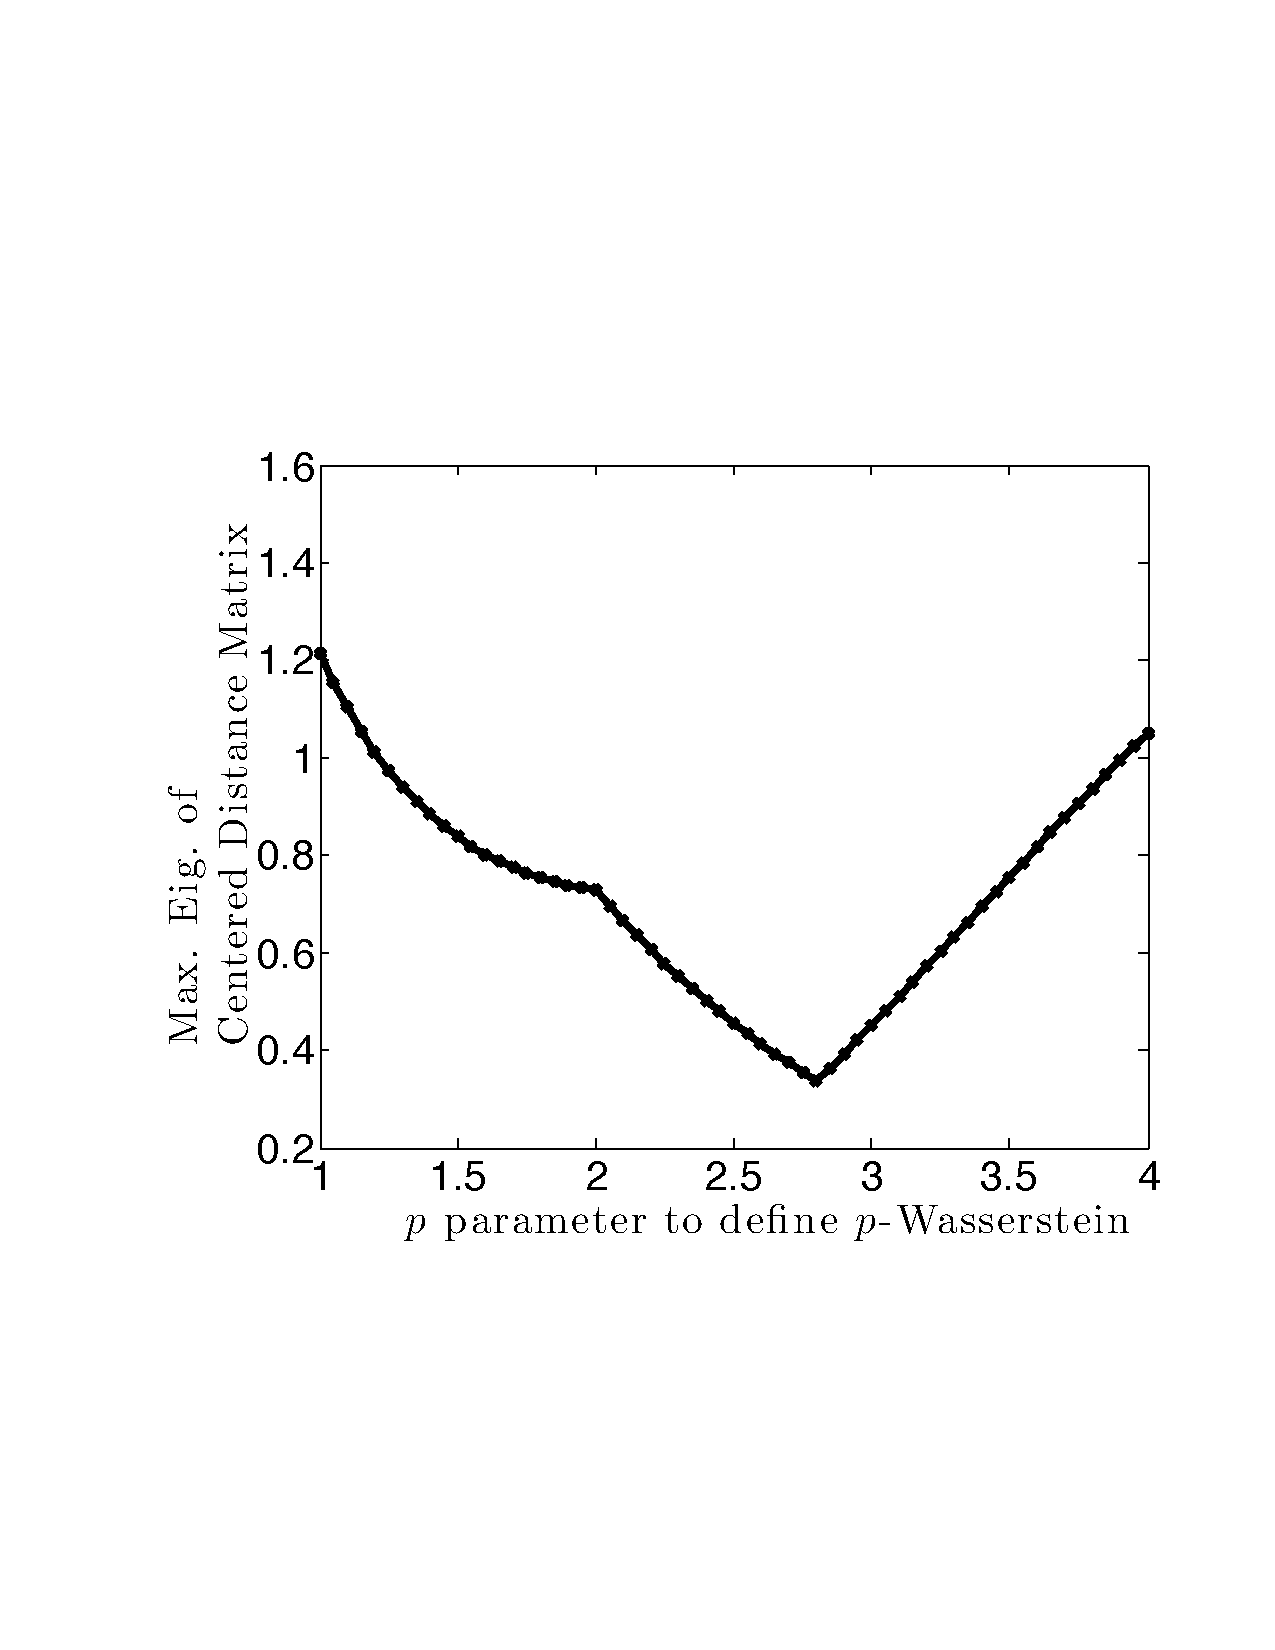
\includegraphics[width=.6\linewidth]{counterexample_nsdness/maxeig_vs_p}
\caption{\label{fig-counterexample}
One can show that a distance is \emph{not} Hilbertian by looking at the spectrum of the centered matrix $\J \D_p^2 \J$ corresponding to the pairwise squared-distance matrix $\D_p^2$ of a set of points. The spectrum of such a matrix is necessarily non-positive if the distance is Hilbertian. Here we plot the values of the maximal eigenvalue of that matrix for points selected in the proof of Proposition~\ref{prop-negative-definite-negative}. We do so for varying values of $p$, and display the maximal eigenvalues we obtain. These eigenvalues are all positive, which shows that for all these values of $p$, the $p$-Wasserstein distance is not Hilbertian.
}
\end{figure}



%%%%%%%%%%%%%%%%%%%%%%%%%%%%%%%%%%%%%%%%%%%%%%%%%%%%%%%%%%%%%%%%%%%%%%%%%%%%%%%%%%%%%%%%%%%%%%%%%%%%
\subsection{Embeddings and Distortion}

An important body of work quantifies the hardness of approximating Wasserstein distances using Hilbertian embeddings. 
%
It has been shown that embedding measures in $\ell_2$ spaces incurs necessarily an important \todoK{need to be more precise here} distortion~(\citet{naor-2005,andoni2015snowflake}) as soon as $\X=\RR^\dim$ with $\dim\geq 2$.

It is possible to embed quasi-isometrically $p$-Wasserstein spaces for $0 < p \leq 1$ in $\ell_1$ (see~\citep{indyk,andoni2008earth,do2011sublinear}), but the equivalence constant between the distances grows fast with the dimension $\dim$. Note also that for $p=1$ the embedding is true only for discrete measures (\ie the embedding constant depends on the minimum distance between the spikes).  \todoK{need to be more precise here} 
%
A closely related embedding technique consists in using the characterization of $\Wass_1$ as the dual of Lipschitz functions $f$ (see~\S\ref{sec-w1-eucl}) and approximating the Lipschitz constraint $\norm{\nabla f}_1 \leq 1$ by a weighted $\ell_1$ ball over the wavelets coefficients; see~\citep{shirdhonkar2008approximate}. 
%
This weighted $\ell_1$ ball of wavelet coefficients defines a so-called Besov space of negative index~\citep{leeb2016holder}.
%
These embedding results are also similar to the bound on the Wasserstein distance obtained using dyadic partitions; see~\citep[Prop. 1]{weed2017sharp} and also~\citep{fournier2015rate}.
%
This also provides a quasi-isometric embedding in $\ell_1$ (this embedding being given by rescaled wavelet coefficients) and comes with the advantage that this embedding can be computed approximately in linear time when the input measures are discretized on uniform grids. We refer to~\citep{mallat2008wavelet} for more details on wavelets. Note that the idea of using multiscale embeddings to compute Wasserstein-like distances has been used extensively in computer vision; see, for instance,~\citep{ling2006diffusion,grauman2005pyramid,CuturiNIPS2006,lazebnik2006beyond}. 

%%%%%%%%%%%%%%%%%%%%%%%%%%%%%%%%%%%%%%%%%%%%%%%%%%%%%%%%%%%%%%%%%%%%%%%%%%%%%%%%%%%%%%%%%%%%%%%%%%%%
\subsection{Negative/Positive Definite Variants of Optimal Transport}

We show later in~\S\ref{sec-sliced} that the \emph{sliced} approximation to Wasserstein distances, essentially a sum of 1-D directional transportation distance computed on random push-forwards of measures projected on lines, is negative definite as the sum of negative definite functions~\citep[\S 3.1.11]{berg84harmonic}. This result can be used to define a positive definite kernel~\citep{kolouri2016sliced}. Another way to recover a positive definite kernel is to cast the optimal transport problem as a soft-min problem (over all possible transportation tables) rather than a minimum, as proposed by~\citet{kosowsky1994invisible} to introduce entropic regularization. That soft-min defines a term whose neg-exponential (also known as a generating function) is positive definite~\citep{cuturi2012positivity}.





%%%%%%%%%%%%%%%%%%%%%%%%%%%%%%%%%%%%%%%%%%%%%%%%%%%%%%%%%%%%%%%%%%%%%%%%%%%%%%%%%%%%%%%%%%%%%%%%%%%%
%%%%%%%%%%%%%%%%%%%%%%%%%%%%%%%%%%%%%%%%%%%%%%%%%%%%%%%%%%%%%%%%%%%%%%%%%%%%%%%%%%%%%%%%%%%%%%%%%%%%
%%%%%%%%%%%%%%%%%%%%%%%%%%%%%%%%%%%%%%%%%%%%%%%%%%%%%%%%%%%%%%%%%%%%%%%%%%%%%%%%%%%%%%%%%%%%%%%%%%%%
\section{Empirical Estimators for OT, MMD and $\phi$-divergences}
\label{sec-empirical-wass}

In an applied setting, given two input measures $(\al,\be) \in \Mm_+^1(\X)^2$, an important statistical problem is to approximate the (usually unknown) divergence $D(\al,\be)$ using only samples $(x_i)_{i=1}^n$ from $\al$ and $(y_j)_{j=1}^m$ from $\be$. These samples are assumed to be independently identically distributed from their respective distributions. 

%%%%%%%%%%%%%%%%%%%%%%%%%%%%%%%%%%%%%%%%%%%%%%%%%%%%%%%%%%%%%%%%%%%%%%%%%%
\subsection{Empirical Estimators for OT and MMD}

For both Wasserstein distances $\Wass_p$ (see~\ref{eq-defn-wass-dist}) and MMD norms (see \S\ref{sec-dual-norms}), a straightforward estimator of the unknown distance between distriubtions is compute it directly between the empirical measures, hoping ideally that one can control the rate of convergence of the latter to the former,
\eq{
	D(\al,\be) \approx D(\hat \al_n,\hat \be_m) \qwhereq
	\choice{
		\hat \al_n \eqdef \frac{1}{n}\sum_i \de_{x_i},\\ 
		\hat \be_m \eqdef \frac{1}{m}\sum_j \de_{y_j}.
	}
}
Note that here both $\hat \al_n$ and $\hat \be_m$ are random measures, so $D(\hat \al_n,\hat \be_m)$ is a random number. 
% 
For simplicity, we assume that $\X$ is compact (handling unbounded domain requires extra constraints on the moments of the input measures).

For such a dual distance that metrizes the weak convergence (see Definition~\ref{dfn-weak-conv}), since there is the weak convergence $\hat\al_n \rightarrow \al$, one has $D(\hat \al_n,\hat \be_n) \rightarrow D(\al,\be)$ as $n \rightarrow +\infty$.
%
But an important question is the speed of convergence of $D(\hat \al_n,\hat \be_n)$ toward $D(\al,\be)$, and this rate is often called the ``sample complexity'' of $D$. 

Note that for $D(\al,\be) = \norm{\cdot}_{\TV}$, since the TV norm does not metrize the weak convergence, $\norms{\hat \al_n - \hat \be_n}_{\TV}$ is not a consistent estimator, namely it does not converge toward $\norm{\al-\be}_{\TV}$. Indeed, with probability 1, $\norms{\hat \al_n - \hat \be_n}_{\TV}=2$ since the support of the two discrete measures does not overlap. Similar issues arise with other $\phi$-divergences, which cannot be estimated using divergences between empirical distributions.


%%%%
\paragraph{Rates for OT.}

For $\X=\RR^\dim$ and measure supported on bounded domain, it is shown by~\citep{dudley1969speed} that for $\dim>2$, and $1 \leq p < +\infty$,  
\eq{
	\EE( |\Wass_p(\hat \al_n,\hat \be_n)-\Wass_p(\al,\be)| ) = O(n^{-\frac{1}{\dim}}),
}
where the expectation $\EE$ is taken with respect to the random samples $(x_i,y_i)_i$. This rate is tight in $\RR^\dim$ if one of the two measures has a density with respect to the Lebesgue measure. This result was proved for general metric spaces~\citep{dudley1969speed} using the notion of covering numbers and was later refined, in particular for $\X=\RR^d$ in~\citep{dereich2013constructive,fournier2015rate}. 
% Proof on $\Wass_1$ implies on $\Wass_p$ for $1 \leq p < +\infty$ by monotonicity in $p$.
This rate can be refined when the measures are supported on low-dimensional subdomains:~\citet{weed2017sharp} show that, indeed, the rate depends on the intrinsic dimensionality of the support. \citeauthor{weed2017sharp} also study the nonasymptotic behavior of that convergence, such as for measures which are discretely approximated (\emph{e.g.} mixture of Gaussians with small variances).
%
It is also possible to prove concentration of $\Wass_p(\hat \al_n,\hat \be_n)$ around its mean $\Wass_p(\al,\be)$; see~\citep{bolley2007quantitative,boissard2011simple,weed2017sharp}.

%%%
\paragraph{Rates for MMD.}

For weak norms $\norm{\cdot}^2_{\Krkhs}$ which are dual of RKHS norms (also called MMD), as defined in~\eqref{eq-kernel-dual}, and contrary to Wasserstein distances, the sample complexity does not depend on the ambient dimension 
\eq{
	\EE( |\norms{\hat \al_n-\hat \be_n}_{\Krkhs} - \norm{\al-\be}_{\Krkhs} | ) = O(n^{-\frac{1}{2}}); 
}
see~\citep{sriperumbudur2012empirical}. 
%
Figure~\ref{fig-sample-complexity} shows a numerical comparison of the sample complexity rates for Wasserstein and MMD distances.  
%
Note, however, that $\norms{\hat \al_n-\hat \be_n}_{\Krkhs}^2$ is a slightly biased estimate of $\norm{\al-\be}_{\Krkhs}^2$. In order to define an unbiased estimator, and thus to be able to use, for instance, SGD when minimizing such losses, one should rather use the unbiased estimator 
\begin{align*}
	\text{MMD}_{\Krkhs}(\hat \al_n,\hat \be_n)^2 & \eqdef
		\frac{1}{n(n-1)} \sum_{i,i'} \Krkhs(x_i,x_{i'})	+
		\frac{1}{n(n-1)}\sum_{j,j'} \Krkhs(y_j,y_{j'}) \\
		 & \qquad - 2
		\frac{1}{n^2}\sum_{i,j} \Krkhs(x_i,y_j), 
\end{align*}
which should be compared to~\eqref{eq-mmd-discr}. It satisfies $\EE(\text{MMD}_{\Krkhs}(\hat \al_n,\hat \be_n)^2) = \norm{\al-\be}_{\Krkhs}^2$; see~\citep{gretton2012kernel}.


\begin{figure}[h!]
\centering
\begin{tabular}{@{}c@{\hspace{1mm}}c@{}}
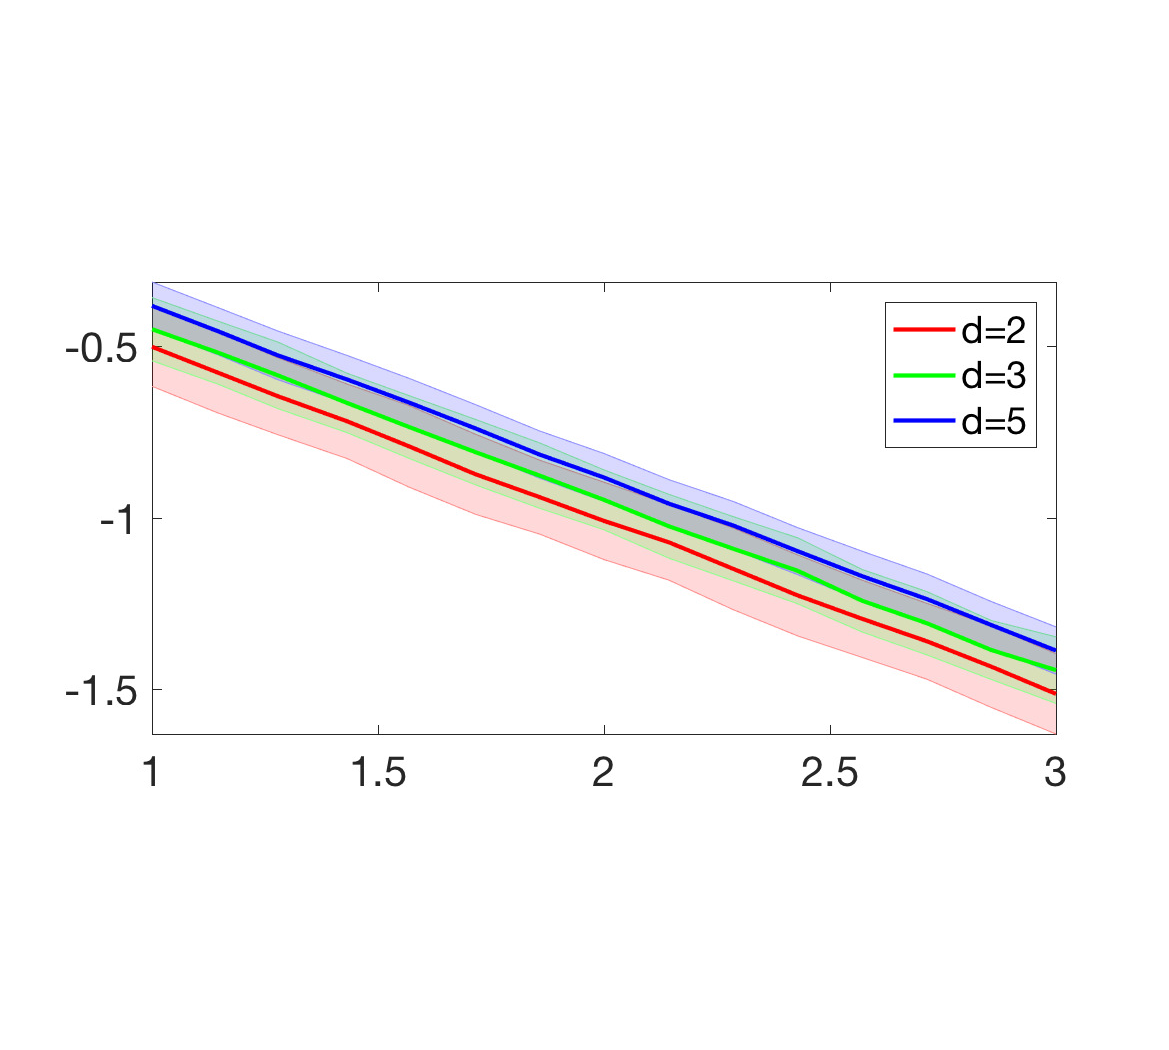
\includegraphics[width=.49\linewidth]{sample-complexity/energy-rates-cropped}&
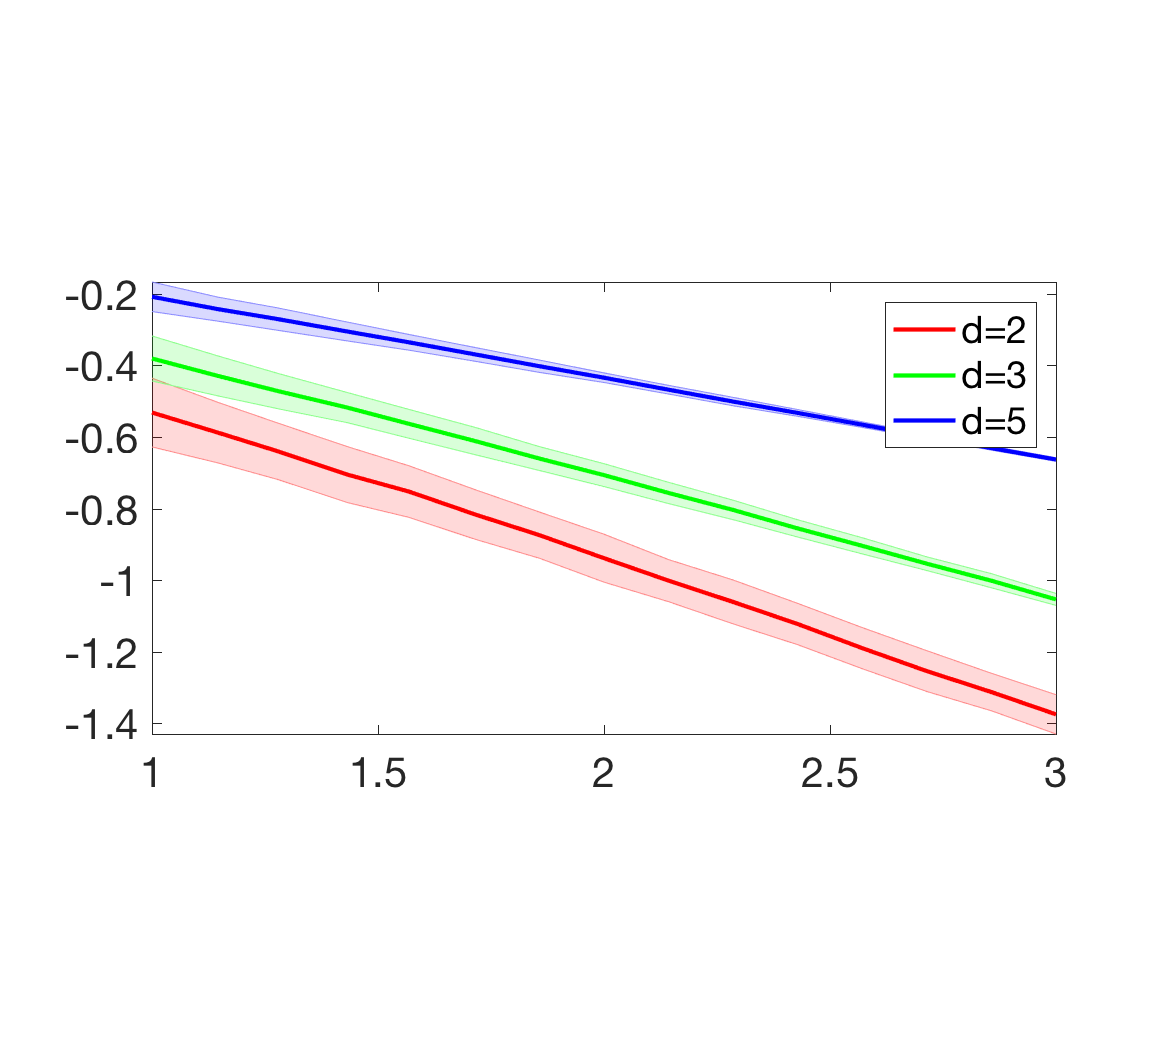
\includegraphics[width=.49\linewidth]{sample-complexity/wass2-rates-cropped}\\
Energy distance $\norm{\cdot}_{H^{-1}}$ & $\Wass_2$ 
\end{tabular}
\caption{\label{fig-sample-complexity}
Decay of $\log_{10}(D(\hat\al_n,\hat\al_n'))$ as a function of $\log_{10}(n)$ for $D$ being the energy distance $D=\norm{\cdot}_{H^{-1}}$ (\ie the $H^{-1}$ norm) as defined in Example~\ref{exp-energy-dist} (left) and the Wasserstein distance $D=\Wass_2$ (right).
%
Here $(\hat\al_n,\hat\al_n')$ are two independent empirical distributions of $\al$, the uniform distribution on the unit cube $[0,1]^\dim$, tested for several value of $\dim \in \{2,3,5\}$.
% 
The shaded bar displays the confidence interval at $\pm$ the standard deviation of $\log(D(\hat\al_n,\al))$. 
}
\end{figure}



%%%%%%%%%%%%%%%%%%%%%%%%%%%%%%%%%%%%%%%%%%%%%%%%%%%%%%%%%%%%%%%%%%%%%%%%%%
\subsection{Empirical Estimators for $\phi$-divergences}

It is not possible to approximate $\Divergm_\phi(\al|\be)$, as defined in~\eqref{def_divergence}, from discrete samples using $\Divergm_\phi(\hat \al_n|\hat \be_n)$. Indeed, this quantity is either $+\infty$ (for instance, for the $\KL$ divergence) or is not converging to $\Divergm_\phi(\al|\be)$ as $n \rightarrow +\infty$ (for instance, for the $\TV$ norm).
%
Instead, it is required to use a density estimator to somehow smooth the discrete empirical measures and replace them by densities; see~\citep{silverman1986density}. 
%
In a Euclidean space $\Xx=\RR^\dim$, introducing $h_\si=h(\cdot/\si)$ with a smooth windowing function and a bandwidth $\si>0$, a density estimator for $\al$ is defined using a convolution against this kernel, 
\eql{\label{eq-kernel-density-estimate}
	\hat \mu_n \star h_\si = \frac{1}{n}\sum_i h_\si(\cdot-x_i).
} 
%
One can then approximate the $\phi$ divergence using
\eq{
	\Divergm_\phi^\si(\hat \al_n |\hat \be_n)
	\eqdef
	\frac{1}{n} \sum_{j=1}^n
	\phi\pa{
		\frac{
			\sum_i h_\si(y_j-x_i)
		}{
			\sum_{j'} h_\si(y_j-y_{j'}),		
		}
	}
} 
where $\si$ should be adapted to the number $n$ of samples and to the dimension $\dim$. 
%
It is also possible to devise nonparametric estimators, bypassing the choice of a fixed bandwidth $\si$ to select instead a number $k$ of nearest neighbors. These methods typically make use of the distance between nearest neighbors~\citep{loftsgaarden1965nonparametric}, which is similar to locally adapting the bandwidth $\si$ to the local sampling density. Denoting $\De_k(x)$ the distance between $x \in \RR^\dim$ and its $k$th nearest neighbor among the $(x_i)_{i=1}^n$, a density estimator is defined as
\eql{\label{eq-knn-density-estimate}
	\rho_{\hat \al_n}^k(x) \eqdef \frac{k/n}{ |B_\dim| \De_k(x)^r },
}
where $|B_\dim|$ is the volume of the unit ball in $\RR^\dim$.
%
Instead of somehow ``counting'' the number of sample falling in an area of width $\si$ in~\eqref{eq-kernel-density-estimate}, this formula~\eqref{eq-knn-density-estimate} estimates the radius required to encapsulate $k$ samples. Figure~\ref{fig-density-estimation} compares the estimators~\eqref{eq-kernel-density-estimate} and~\eqref{eq-knn-density-estimate}.
%
A typical example of application is detailed in~\eqref{eq-discr-entropy} for the entropy functional, which is the KL divergence with respect to the Lebesgue measure. We refer to~\citep{BerishaHero} for more details.


\newcommand{\myFigDE}[1]{\includegraphics[width=.32\linewidth]{density-estimation/#1}}

\begin{figure}[h!]
\centering
\begin{tabular}{@{}c@{\hspace{1mm}}c@{\hspace{1mm}}c@{}}
\myFigDE{kernel-1} & \myFigDE{kernel-3} & \myFigDE{kernel-5} \\
$\si=2.5 \cdot 10^{-3}$ & $\si=15 \cdot 10^{-3}$ & $\si=25 \cdot 10^{-3}$ \\
\myFigDE{nn-1} & \myFigDE{nn-3} & \myFigDE{nn-5} \\
$k=1$ & $k=50$ & $k=100$
\end{tabular}
\caption{\label{fig-density-estimation}
Comparison of kernel density estimation $\hat \mu_n \star h_\si$ (top, using a Gaussian kernel $h$) and $k$-nearest neighbors estimation $\rho_{\hat \al_n}^k$ (bottom) for $n=200$ samples from a mixture of two Gaussians.
}
\end{figure}



%%%%%%%%%%%%%%%%%%%%%%%%%%%%%%%%%%%%%%%%%%%%%%%%%%%%%%%%%%%%%%%%%%%%%%%%%%%%%%%%
%%%%%%%%%%%%%%%%%%%%%%%%%%%%%%%%%%%%%%%%%%%%%%%%%%%%%%%%%%%%%%%%%%%%%%%%%%%%%%%%
%%%%%%%%%%%%%%%%%%%%%%%%%%%%%%%%%%%%%%%%%%%%%%%%%%%%%%%%%%%%%%%%%%%%%%%%%%%%%%%%
\section{Entropic Regularization: Between OT and MMD}
\label{sec-entropy-ot-mmd}

Following Proposition~\ref{prop-sinkhorn-div}, we recall that the Sinkhorn divergence is defined as 
\eq{
	\SINKHORNP_\C^\varepsilon(\a,\b) \eqdef 
	\dotp{\P^\star}{\C} = 
	\dotp{e^{\frac{\fD^\star}{\varepsilon}}}{(\K\odot \C)e^{\frac{\gD^\star}{\varepsilon}}},
}
where $\P^\star$ is the solution of~\eqref{eq-regularized-discr} while $(\fD^\star,\gD^\star)$ are solutions of~\eqref{eq-dual-formulation}.
%
Assuming $\C_{i,j}=\dist(x_i,x_j)^p$ for some distance $\dist$ on $\X$, for two discrete probability distributions of the form~\eqref{eq-pair-discr}, this defines a regularized Wasserstein cost
\eq{
	\Wass_{p,\varepsilon}(\al,\be)^p \eqdef \SINKHORNP_\C^\varepsilon(\a,\b).
}
This definition is generalized to any input distribution (not necessarily discrete) as
\eq{
	\Wass_{p,\varepsilon}(\al,\be)^p \eqdef \int_{\X \times \X} \dist(x,y)^p \d\pi^\star(x,y),
}	
where $\pi^\star$ is the solution of~\eqref{eq-entropic-generic}. 

In order to cancel the bias introduced by the regularization (in particular, $\Wass_{p,\varepsilon}(\al,\al) \neq 0$), we introduce a corrected regularized divergence
\eq{
	\tilde\Wass_{p,\varepsilon}(\al,\be)^p \eqdef
	2 \Wass_{p,\varepsilon}(\al,\be)^p
	-
	\Wass_{p,\varepsilon}(\al,\al)^p
	-
	\Wass_{p,\varepsilon}(\be,\be)^p.
}
It is proved in~\citep{feydy2018interpolating} that if $e^{-c/\epsilon}$ is a positive kernel, then a related corrected divergence (obtained by using $\MKD_\C^\varepsilon$ in place of $\SINKHORNP_\C^\varepsilon$) is positive. 
%
Note that it is possible to define other renormalization schemes using regularized optimal transport, as proposed, for instance, by~\citet{amari2017information}.

\begin{figure}[h!]
\centering
\begin{tabular}{@{}c@{\hspace{1mm}}c@{}}
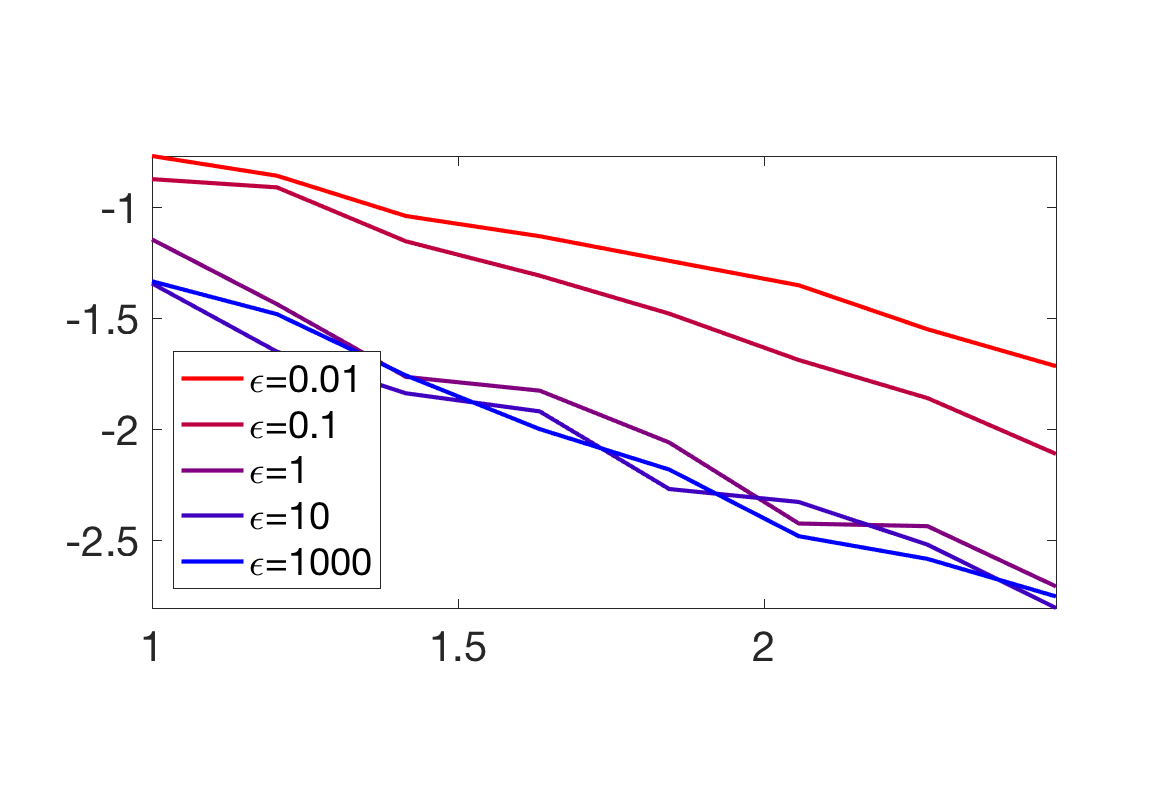
\includegraphics[width=.49\linewidth]{sample-complexity-regul/influ-epsilon-d2-cropped}&
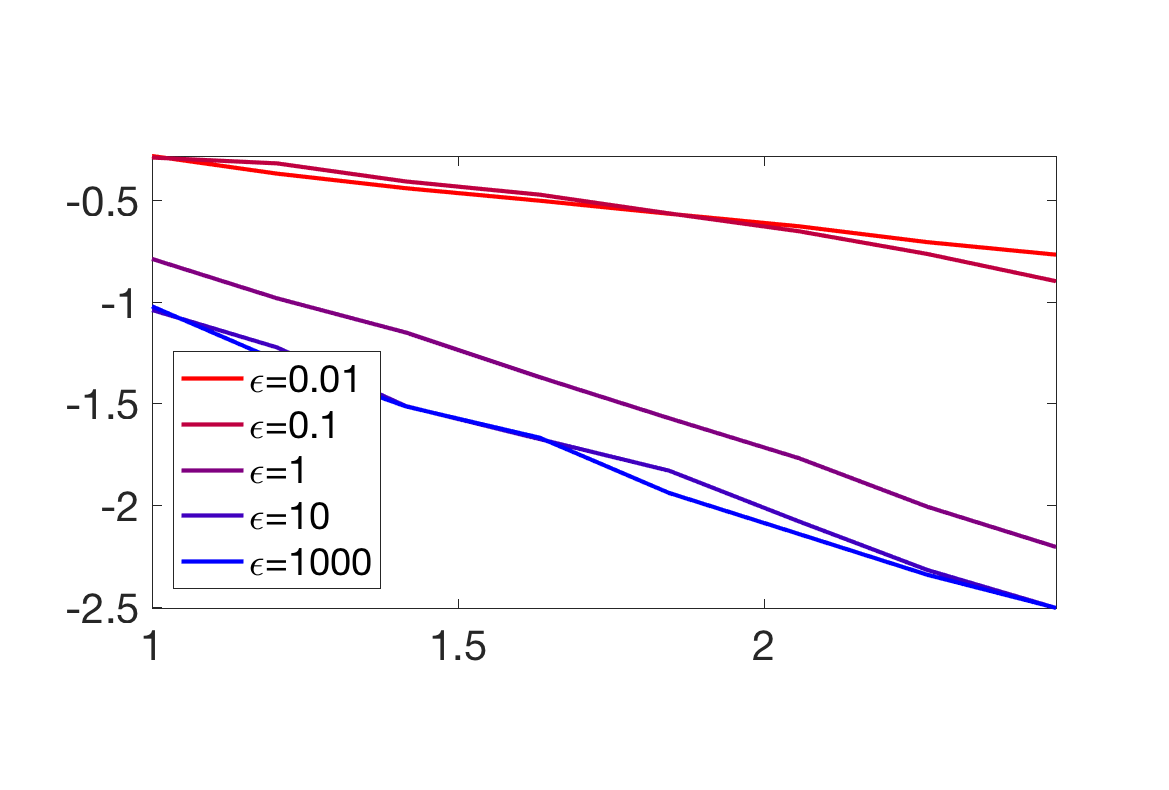
\includegraphics[width=.49\linewidth]{sample-complexity-regul/influ-epsilon-d5-cropped}\\
$\dim=2$ & $\dim=5$
\end{tabular}
\caption{\label{fig-sample-complexity-regul}
Decay of $\EE(\log_{10}(\tilde\Wass_{p,\varepsilon}(\hat\al_n,\hat\al_n')))$, for $p=3/2$ for various $\varepsilon$, as a function of $\log_{10}(n)$ where $\al$ is the same as in Figure~\ref{fig-sample-complexity}. \todoK{redo the plot with higher precision}
}
\end{figure}


The following proposition, whose proof can be found in~\citep{ramdas2017wasserstein}, shows that this regularized divergence interpolates between the Wasserstein distance and the energy distance defined in Example~\ref{exp-energy-dist}.

\begin{prop}
	One has
	\eq{
		\tilde\Wass_{p,\varepsilon}(\al,\be)  \overset{\varepsilon \rightarrow 0}{\longrightarrow} 2 \Wass_{p}(\al,\be)
		\qandq
		\tilde\Wass_{p,\varepsilon}(\al,\be)^p \overset{\varepsilon \rightarrow +\infty}{\longrightarrow} \norm{\al-\be}_{\text{ED}(\X,\dist)}^2, 
	}
	where $\norm{\cdot}_{\text{ED}(\X,\dist)}$ is defined in~\eqref{eq-defn-ed}. 
\end{prop}

Figure~\ref{fig-sample-complexity-regul} shows numerically the impact of $\epsilon$ on the sample complexity rates. It is proved in~\cite{genevay2018sample}, in the case of $c(x,y)=\norm{x-y}^2$ on $\Xx=\RR^d$, that these rates interpolate between the ones of OT and MMD. 





